% CVPR 2025 Paper Template; see https://github.com/cvpr-org/author-kit

\documentclass[10pt,twocolumn,letterpaper]{article}

%%%%%%%%% PAPER TYPE  - PLEASE UPDATE FOR FINAL VERSION
\usepackage{cvpr}              % To produce the CAMERA-READY version
\usepackage{cvpr}
% \usepackage[review]{cvpr}      % To produce the REVIEW version
% \usepackage[pagenumbers]{cvpr} % To force page numbers, e.g. for an arXiv version

% Import additional packages in the preamble file, before hyperref
%
% --- inline annotations
%
\newcommand{\red}[1]{{\color{red}#1}}
\newcommand{\todo}[1]{{\color{red}#1}}
\newcommand{\TODO}[1]{\textbf{\color{red}[TODO: #1]}}
% --- disable by uncommenting  
% \renewcommand{\TODO}[1]{}
% \renewcommand{\todo}[1]{#1}



% It is strongly recommended to use hyperref, especially for the review version.
% hyperref with option pagebackref eases the reviewers' job.
% Please disable hyperref *only* if you encounter grave issues, 
% e.g. with the file validation for the camera-ready version.
%
% If you comment hyperref and then uncomment it, you should delete *.aux before re-running LaTeX.
% (Or just hit 'q' on the first LaTeX run, let it finish, and you should be clear).
\definecolor{cvprblue}{rgb}{0.21,0.49,0.74}
\usepackage[pagebackref,breaklinks,colorlinks,allcolors=cvprblue]{hyperref}

%%%%%%%%% PAPER ID  - PLEASE UPDATE
\def\paperID{69} % *** Enter the Paper ID here
\def\confName{CVPR}
\def\confYear{2025}

%%%%%%%%% TITLE - PLEASE UPDATE
\title{Detecting Toxic Content from Social Media using LLMs}

%%%%%%%%% AUTHORS - PLEASE UPDATE
% \author{First Author\\
% Institution1\\
% Institution1 address\\
% {\tt\small firstauthor@i1.org}
% % For a paper whose authors are all at the same institution,
% % omit the following lines up until the closing ``}''.
% % Additional authors and addresses can be added with ``\and'',
% % just like the second author.
% % To save space, use either the email address or home page, not both
% \and
% Second Author\\
% Institution2\\
% First line of institution2 address\\
% {\tt\small secondauthor@i2.org}
% }

\author{
  Naman Chhibbar \\
  {\tt \small ma21btech11011@iith.ac.in}
  \and
  Shubham Vishwakarma \\
  {\tt \small ma21btech11020@iith.ac.in}
  \and
  Kaustubh Dandegaonkar \\
  {\tt \small ma21btech11003@iith.ac.in}
  \and
  Saradhi Kartheek \\
  {\tt \small ma21btech11015@iith.ac.in}
  \and
  Manoj Kumar \\
  {\tt \small es21btech11010@iith.ac.in}
}

\affiliation{ab}

\begin{document}
\maketitle

\begin{abstract}

\begin{quote}

\textbf{Prior warning to readers: This paper contains explicit language and sensitive content.}
    
\end{quote}
    
\end{abstract}

\section{Introduction}

\begin{frame}{Introduction}

\begin{itemize}

    \item Toxicity in natural language refers to expressing hate or stereotypes towards an individual or a group of people using language.

    \item In general, toxic content can be categorized into:
    \begin{itemize}
        \item \textbf{Derogation:} Insulting or demeaning a group of individuals.
        \item \textbf{Animosity:} Subtly abusing a group (without using explicit language).
        \item \textbf{Threatening:} Expression of intent to harm, supporting harmful act, or encouraging inflicting harm on an individual or a group.
        \item \textbf{Supporting toxicity:} Encouraging, justifying, or glorifying hateful acts.
        \item \textbf{Dehumanizing:} Treating an individual or a group as "less human" (for example, insects, animals, etc.).
    \end{itemize}

\end{itemize}

\end{frame}

\section{Problem Statement}

Given some social media content (in the form of natural language), we want to predict whether it is toxic; this makes this task a binary classification problem.
Formally speaking, given a natural language input $x = (w_1, w_2, \dots, w_n)$, we need to predict if $x$ is toxic.

\section{Related Works}

\begin{frame}{Related Works}
    \begin{itemize}
        \item 
    \end{itemize}
\end{frame}

\section{Datasets}

\begin{frame}{Datasets}

  \begin{itemize}
  
    \item ToxicGen \citep{hartvigsen2022toxigen}
    \begin{itemize}
      \item Created by prompting an LLM to produce toxic and benign texts.
      \item Texts do not contain explicit language and target minority groups.
      \item Example: Muslims deserve to die.
    \end{itemize}
    
    \item SBIC (Social Bias Inference Corpus) \citep{zhang2024efficient}
    \begin{itemize}
      \item Texts contain stereotypes and offensiveness towards an individual or a group of people.
      \item Example: Women candidates are less qualified.
    \end{itemize}

    \item DHate \citep{vidgen2020learning}
    \begin{itemize}
      \item Details about this dataset are not revealed.
      \item From manual analysis, this dataset seems to be comprised of hate of minorities.
      \item Example: I always feel unsafe when surrounded by Arabs.
    \end{itemize}

  \end{itemize}
    
\end{frame}

\section{Challenges}

\begin{frame}{Challenges}

% \begin{itemize}

%     \item Performance relies heavily on the quality of prompts
%     \item Deploying LLMs for toxic content detection can incur both high run-time costs and high latency 
%     \item \textbf{Existing works}-Bootstrapping and Distilling LLM's
%     \begin{itemize}
%         \item Decision-Tree-of-Thought
%         \item Fine-tune a suitable student LM with a smaller model size
%     \end{itemize}
%     \begin{figure}
%         \centering
%         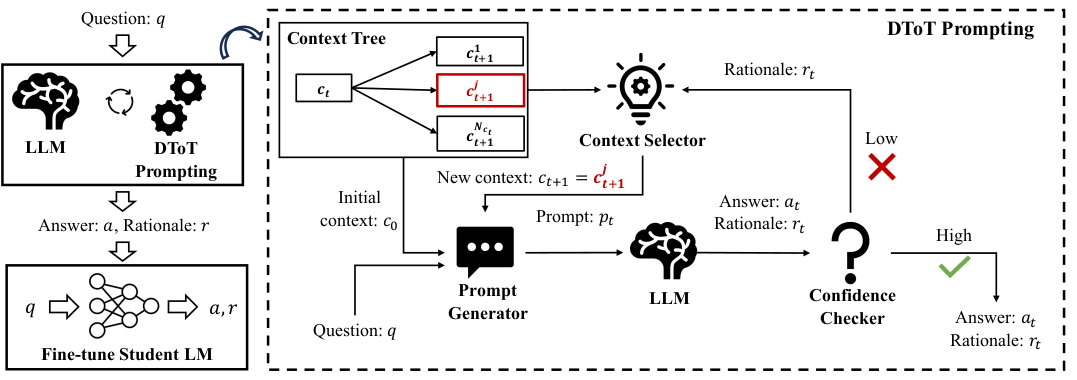
\includegraphics[width=1\linewidth]{images/BD_LLM.png}
%         \caption{Illustration of BD-LLM}
%         \label{fig:1}
%     \end{figure}

% \end{itemize}

\begin{itemize}

    \item A major challenge in detecting toxicity is that toxicity is relative.
    \item Some may think that some content is toxic, while others may not.
    \item This happens due to different perceptions of people.
    \item In addition, the datasets being used are also biased.
    \item For example:
    \begin{itemize}
        \item "I'm going to kill Amy" is labelled as not toxic in the DHate dataset, whereas it falls in the "Threatening" category.
        \item "A dude with money can only impress a broke bitch" is labelled as not toxic in the SBIC dataset, whereas many may think it is (due to vulgarity).
    \end{itemize}

\end{itemize}

\begin{itemize}
    \item 
\end{itemize}

\end{frame}

\section{Proposed Methods}
\subsection{Clustering Based Toxicity Detection
}
\begin{itemize}
    \item This approach maintains a vector database of toxic examples.
    \item When we get a new input, we use the vector database to extract $k$-nearest-neighbors toxic examples.
    \item We then use these examples for $k$-shot prompting. 
    \item For classification, we can either use a transformer with a classifier head or an API call to an LLM (for example, GPT) to get a "yes" or "no" output.
\end{itemize}
\subsection{Toxicity-Attended Roberta Classification}
In this approach, we build upon the architecture of the \textit{unitary/unbiased-toxic-roberta} model, introducing key modifications to enhance its focus on offensive content. While the original model features an attention mechanism in its encoder block, we introduce an additional attention layer specifically designed to attend to the context surrounding offensive language (c.f figure \ref{fig:models-diff}).

For this new attention block, we utilize a curated list of profane words from CMU as the \textbf{queries}, while the \textbf{keys} and \textbf{values} are derived from the embeddings of the input text. This mechanism allows the model to selectively focus on the regions of input that contain or are influenced by toxic language, helping it better capture nuanced context around offensive content.

By incorporating this toxicity-attended attention layer, we aim to improve the model's ability to accurately classify toxic and non-toxic content with heightened sensitivity to harmful language patterns.

\begin{figure}[h]
    \centering
    \begin{subfigure}[b]{0.45\linewidth} 
        \centering
        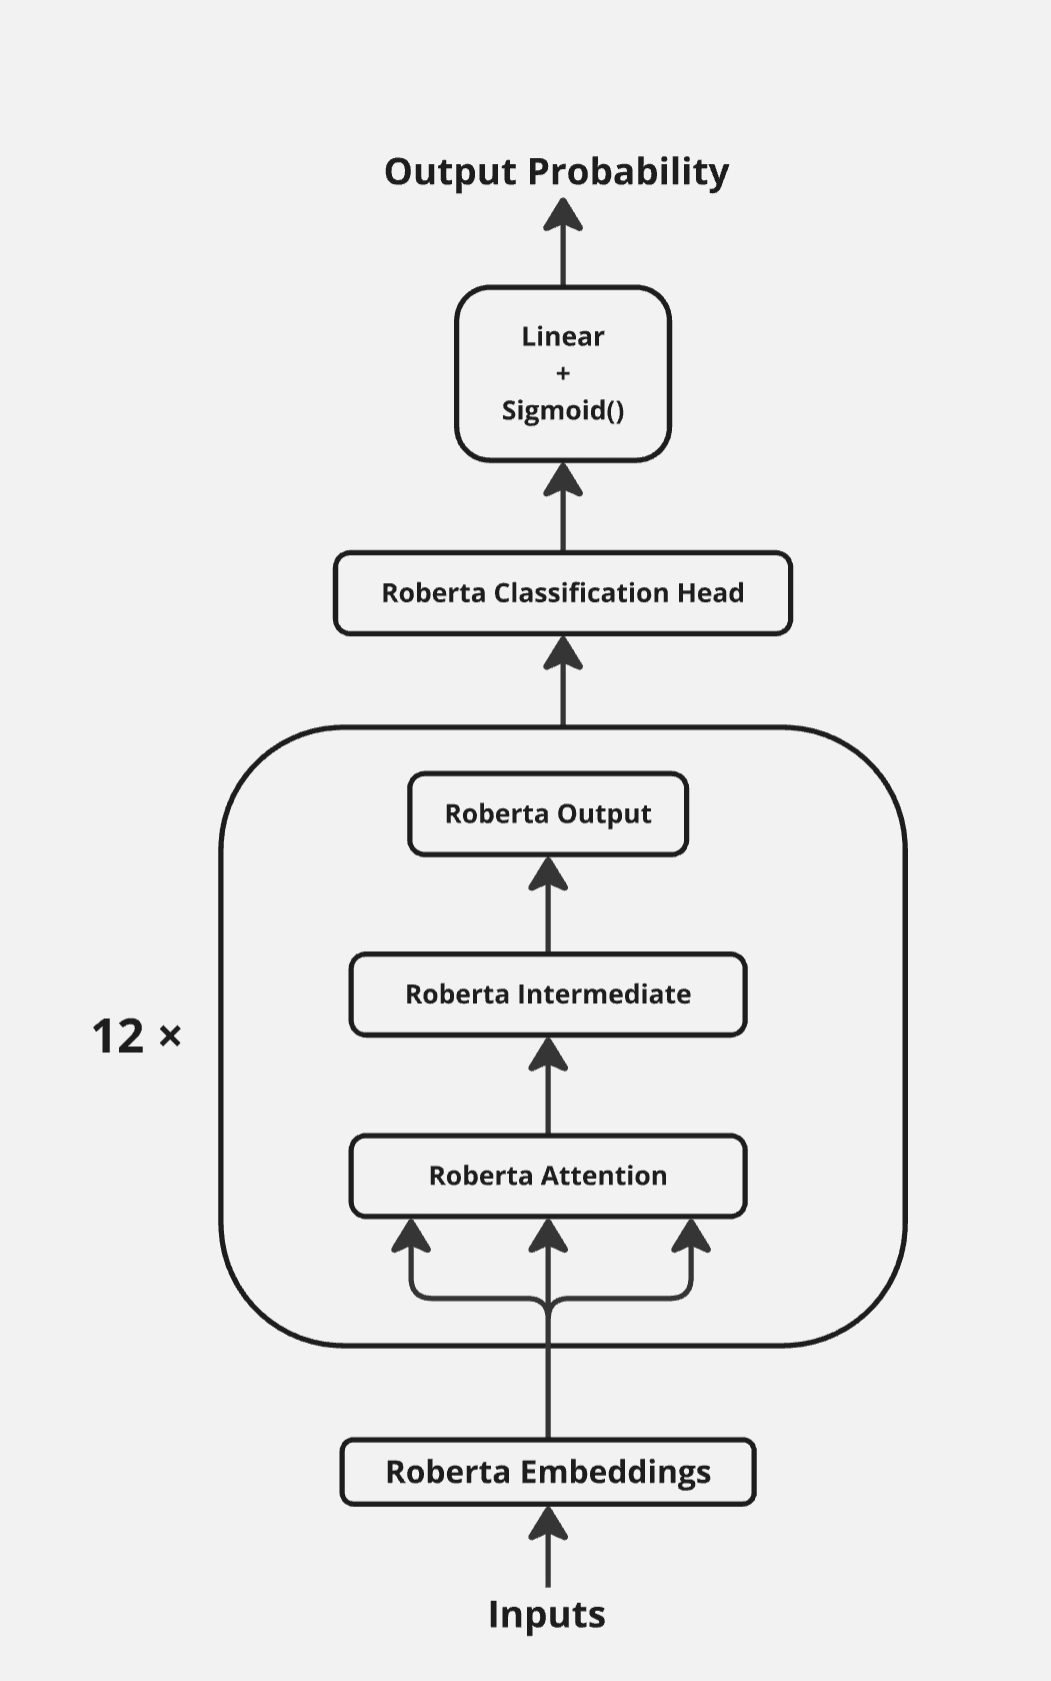
\includegraphics[width=\linewidth]{Images/Screenshot_20241023_113542_Miro.jpg}
        \caption{Original unitary/unbiased-toxic-roberta model}
        \label{fig:org-model}
    \end{subfigure}
    \hfill
    \begin{subfigure}[b]{0.45\linewidth} 
        \centering
        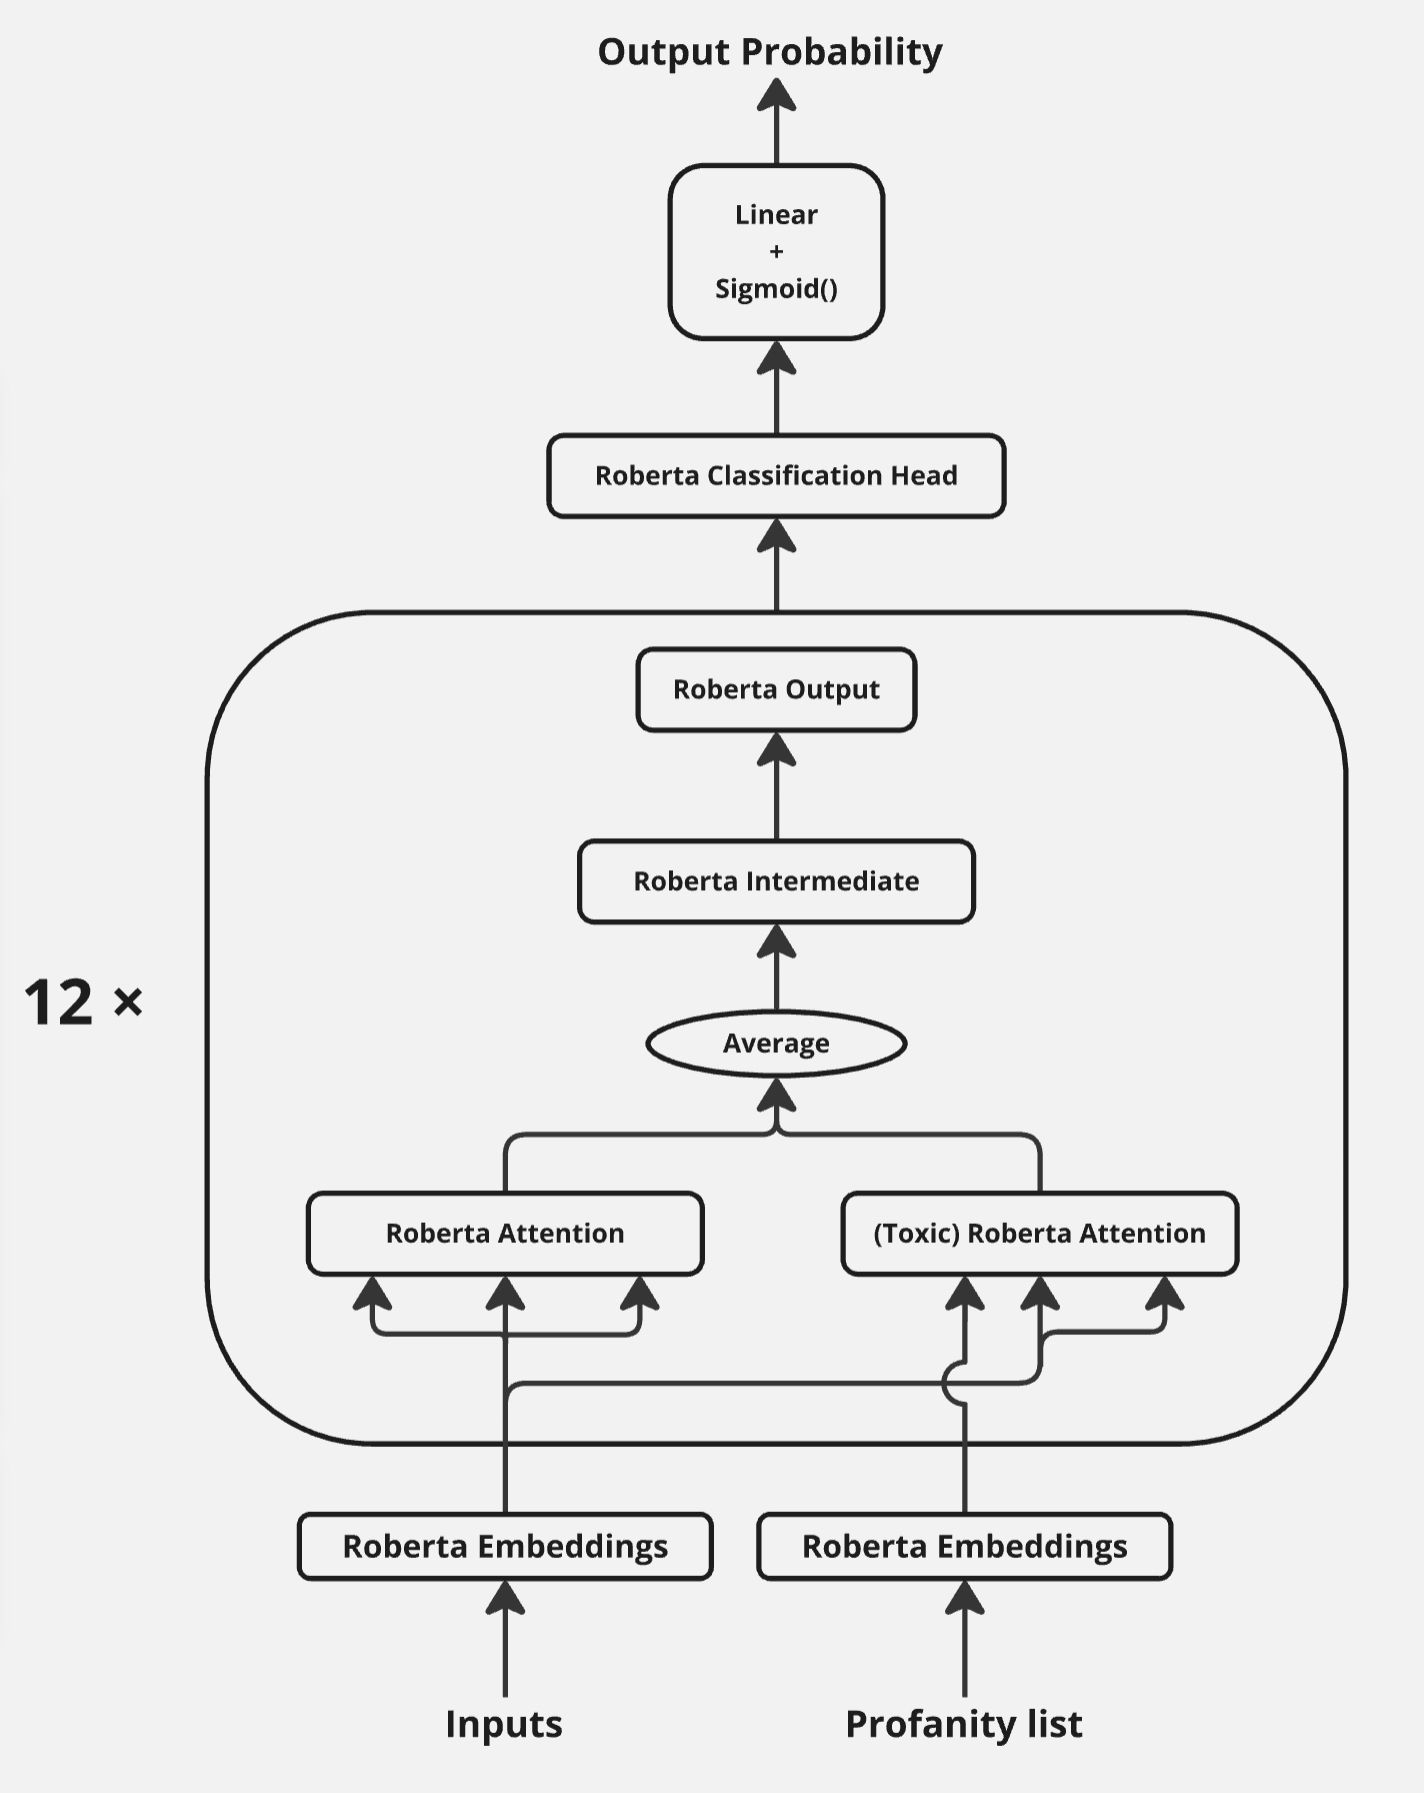
\includegraphics[width=\linewidth]{Images/Screenshot_20241023_113521_Miro.jpg}
        \caption{Toxic-attended roberta model}
        \label{fig:modified-model}
    \end{subfigure}
    
    \caption{Comparison between the original unitary/unbiased-toxic-roberta model and the modified Toxic-attended Roberta model}
    \label{fig:main-figure}
\end{figure}
\section{Conclusion}

To be filled.


\bibliographystyle{ieeenat_fullname}
\bibliography{anthology}

\end{document}
